

\section{Results}
    In this section, we report the outcome of the experiments which we performed with our proposed model. This includes extensive ablation study and  comparison with current state-of-the-art models. All of the evidence points to our model being competitive with other state-of-the-art models, as well as lightweight and cost-effective.
     
     % 	% 	%		%		%		% 	% 	%		%		%		%
     
        \begin{table}[htp]
    \begin{center}
		\begin{tabular}{lc}
			\hline
			Methods     &  Accuracy ($\%$)    \\
			\hline
            2s-MDCN(without skip connection)    &      86.75  \\
            2s-MDCN(with skip connection)    &      87.50 \\
            \hline
		\end{tabular}
    \end{center}
	\caption{Ablation study for the impact of concatenated skip connections on 2s-MDCN.}
    \label{tab:abl_skip}
	\end{table}
	
	
		\begin{table}[htp]
    \begin{center}
		\begin{tabular}{lcc}
			\hline
			Methods    &  Accuracy ($\%$)    \\
			\hline
            2s-MDCN (flow only)   &  80.50  \\
            2s-MDCN (RGB only)    &  87.50 \\
            2s-MDCN (fusion)   & 89.70 \\
            \hline
		\end{tabular}
    \end{center}
	\caption{Ablation study of the performance of 2s-MDCN with respect to input type.}
    \label{tab:abl_frame}
	\end{table}
	
	 % 	% 	%		%		%		% 	% 	%		%		%		%

%  Ablation Study for frame length   %

% 	% 	%		%		%		% 	% 	%		%		%		%

	\begin{table}[htp]
    \begin{center}
		\begin{tabular}{lcc}
			\hline
			Methods     &  Frame Length  &  Accuracy ($\%$)    \\
			\hline
            2s-MDCN   &    16  &  86.30  \\
            2s-MDCN    &    32 &  89.7 \\
            \hline
		\end{tabular}
    \end{center}
	\caption{Ablation study of the performance of 2s-MDCN with respect to frame length.}
    \label{tab:abl_stream}
	\end{table}

\begin{table*}[htb]
    \begin{center}
		\begin{tabular}{lccc}
			\hline
			Methods	                     &\# Params (M)              & Complexity (GFLOPS)                & Accuracy($\%$)		\\
			\hline
            R(2+1)D~\cite{r21dtran2018closer}          					& 33.20 									& 42.42 							  						& 81.25								\\
			C3D~\cite{c3dtran2015learning} 									& 79.90 									& 38.62							   						& 82.75								\\
			ConvLSTM~\cite{29_sudhakaran2017learning} 						& -                                      	& -															& 77.00					\\
			I3D (RGB)~\cite{i3dcarreira2017quo}							& 12.30										& 111.30 													&	85.75						\\
           I3D 	(flow)~\cite{i3dcarreira2017quo}								& 12.30										& 102.52 												&	75.50						\\
           I3D (two-stream)~\cite{i3dcarreira2017quo}	 				& 24.40									& 213.85 												&	81.50						\\
           FlowGate (RGB)~\cite{cheng2019rwf}				& 0.25									& 8.76													& 84.50								\\
           FlowGate (flow)~\cite{cheng2019rwf}				& 0.25									& 8.29													&	75.50							\\
           FlowGate (fusion)~\cite{cheng2019rwf}			 	& 0.27										& 16.98													& 87.25								\\
            \hline
			\textbf{2s-MDCN (flow only)}					& \textbf{0.47}						& \textbf{4.47}								 		& \textbf{80.50}							\\
			\textbf{2s-MDCN (RGB only)}						& \textbf{0.47}						& \textbf{4.47}								 		& \textbf{87.50}							\\
			\textbf{2s-MDCN (fusion)}						& \textbf{0.94}						& \textbf{8.16}								 		& \textbf{89.70}							\\
			\hline
		\end{tabular}		
    \end{center}
	\caption{Comparison of our model with other state-of-the-art methods on RWF-2000 violence dataset.}
    \label{tab:rwf-2000}
	\end{table*}
 \begin{table}[t]
 \caption{Comparison of our model with other state-of-the-art methods on Hockey-fight and Movies-fight dataset.}
    \begin{center}
		\begin{tabular}{lcc}
			\hline
			\multirow{2}{*}{Methods}	 & \multicolumn{2}{c}{Accuracy($\%$)} \\\cline{2-3}
						     									& Hockey   				& 	Movies    \\
			\hline
            ViF~\cite{hassner2012violent_6}           										& 82.9 									& - 								\\
            LHOG+LOF~\cite{lhog_zhou2018violence} 									& 95.1 									& - 								\\
            HOF+HIK~\cite{hog_nievas2011violence} 										& 88.6									& 59.0 								\\
            HOF+HIK~\cite{hog_nievas2011violence} 										& 91.7										& 49.0 								\\
            MoWLD+BoW~\cite{mowd_zhang2017mowld} 								& 91.9										& - 								\\
            MoSFIT+HIK~\cite{hog_nievas2011violence} 								& 90.9									& 89.5							\\
            \hline
             FightNet~\cite{26_zhou2017violent}										& 97.0									& 100							\\
            3D ConvNet~\cite{3dconvnet_song2019novel} 									& 99.62									& 99.9 							\\
            ConvLSTM~\cite{29_sudhakaran2017learning} 									& 97.1										& 100 								\\
            C3D~\cite{c3dtran2015learning} 												& 96.5									& 100 								\\
			I3D (RGB)~\cite{i3dcarreira2017quo} 										& 98.5									& 100 									\\
			I3D (Flow)~\cite{i3dcarreira2017quo} 										& 84.0									& 100 									\\
% 			I3D (Fusion)~\cite{i3dcarreira2017quo} 									& 97.5									& 100 									\\
			FlowGate~\cite{cheng2019rwf}										& 98.0									& 100                               \\
			\hline
			2s-MDCN									& \textbf{99.0}						& \textbf{100}									\\
			\hline
		\end{tabular}		
    \end{center}
    \label{tab:hockey_movie}
	\end{table}
	
     
    \subsection{Ablation Study}
    \label{sec:ablation}
    We performed different ablation studies in order to identify the best hyperparameters, input features and model architecture. 
    
    First, we compared our model without skip connection.  %residual connection is subject to change
    Table~\ref{tab:abl_skip} displays the model accuracy with and without the concatenation of skip connection. 
    Our model achieves ${89.7\%}$ with skip connection and while we turned off the skip connection it drops at ${88.7\%}$.
    The results show that skip connection helps information flow more efficiently and thus helps to improve accuracy.
    
    We also demonstrate the capability of our model with a single input stream. As shown in Table~\ref{tab:abl_stream}, our model achieves 89.7\% accuracy when two different input methods are used. We achieve 87.5\% accuracy while using only RGB stream, and by using only optical flow our model is able to achieve 78.5\% accuracy in RWF-2000 violence detection dataset.
        
    Second, as shown in Table~\ref{tab:abl_frame}, we experimented with different frame lengths and found that frame length of $32$ gives the best accuracy for our model. 
    When we used $16$ frames as input we achieved a score of ${85.3\%}$. 
%    This can be the evidence of the fact that the more information can be provided to a model, the better it will perform.
    
    
    % 	% 	%		%		%		% 	% 	%		%		%		%

%  Comparison with rwf-2000 dataset  %

% 	% 	%		%		%		% 	% 	%		%		%		%
\begin{figure}
    \centering
    \subfigure[Comparison between training and validation accuracy.]
    {
        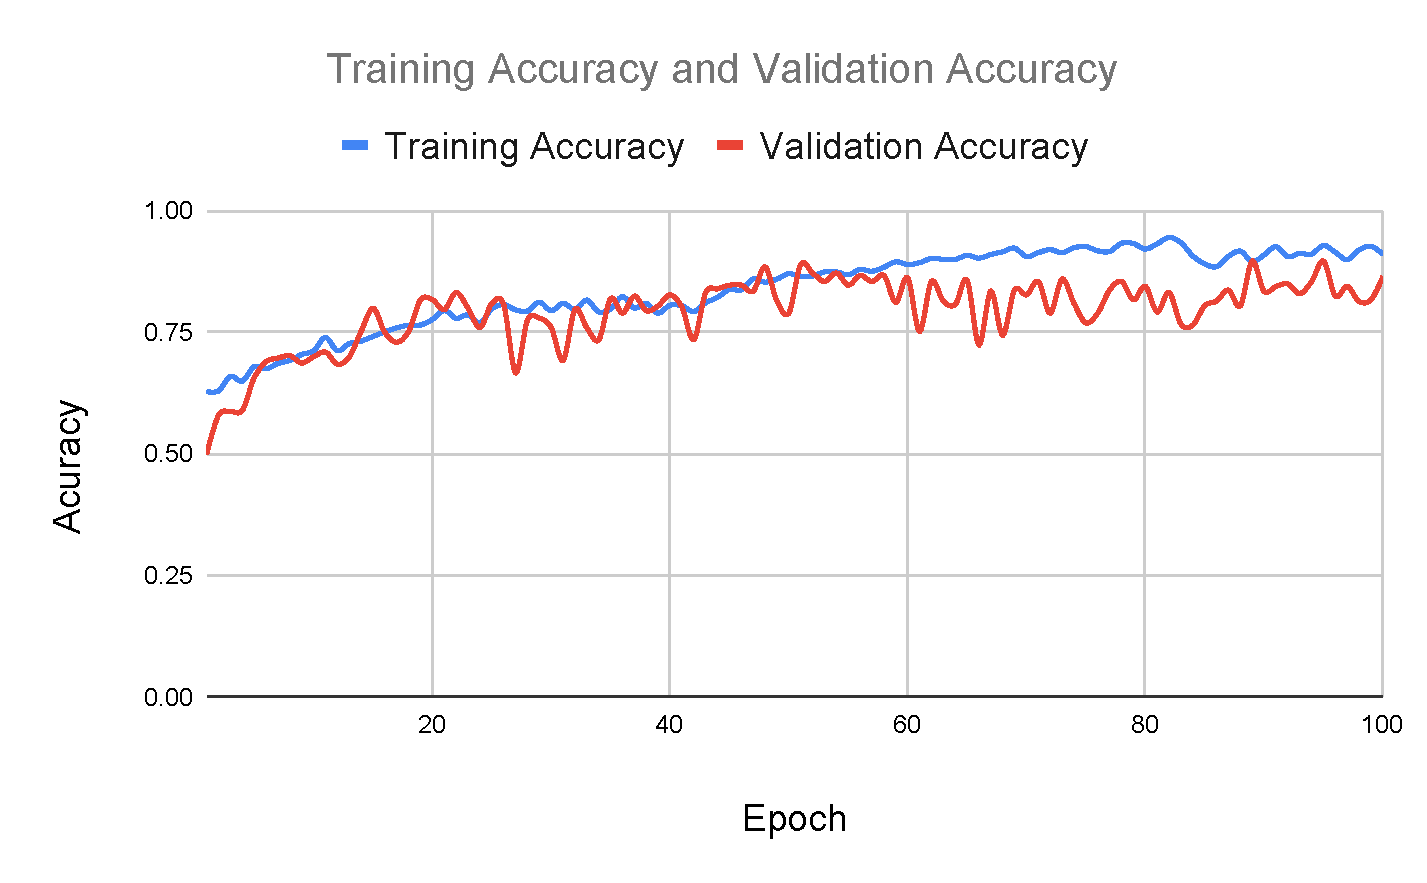
\includegraphics[width=0.9\linewidth]{new_images/accuracy.pdf}
        \label{fig:accuracy}
    }
    \\
    \subfigure[Comparison between training and validation loss]
    {
        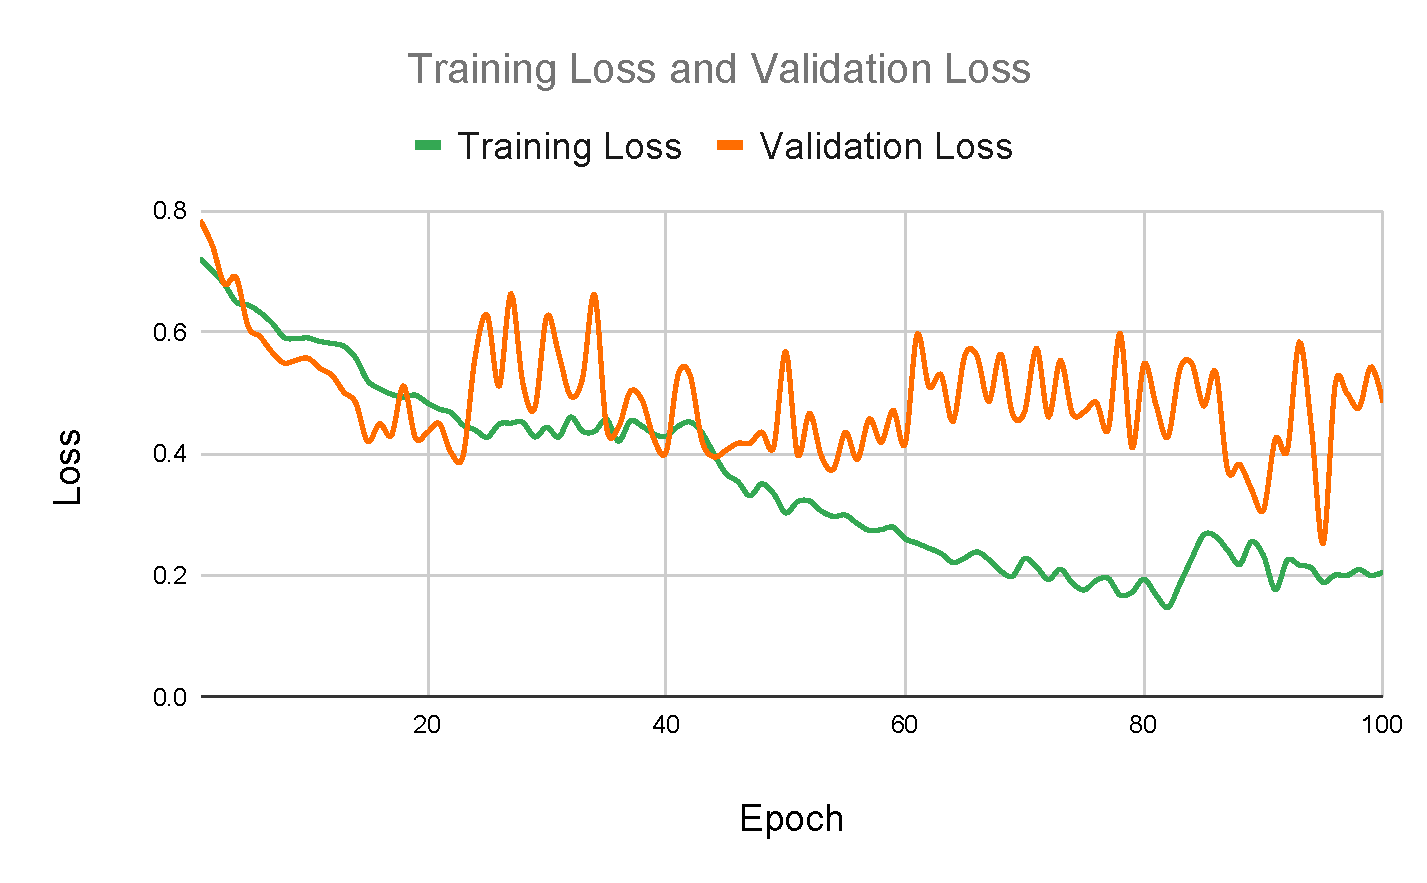
\includegraphics[width=0.9\linewidth]{new_images/loss.pdf}
        \label{fig:loss}
    }
    \caption{Performance measurement between training and validation process.}
    \label{fig:mdcn_train_vs_val}
\end{figure}

	\subsection{Qualitative Analysis}
We illustrate visualization of features from an individual DSTC block and compare with the features from a single 3D CNN layer, which is used as a branch in our model. 
In the Fig.~\ref{fig:features_vis}, we show three consecutive frames of samples from RWF-2000 dataset denoted by $F_{t-1}$, $F_t$, and $F_{t+1}$. 
We also illustrate the features extracted from the first DSTC block and compare them with the single 3D CNN layer. 
From the visualization, it is evident that the combination of 1D, 2D, and 3D CNN layers extract salient features from the input and makes our model efficient and accurate.


    \subsection{Comparison with the state-of-the-art}
    
      In this section, we compare our models with other violence detection state-of-the-art models on the datasets stated earlier.
      
      Table~\ref{tab:hockey_movie} shows the comparison of our model with other models on Hockey-fight and Movie-fight dataset. 
      Our model outperforms the hand-crafted features based models and deep learning-based models as well on both datasets. 
      2s-MDCN obtained ${100.0\%}$ and ${99.0\%}$ accuracy on Hockey-fight dataset and Movies-fight dataset respectively.
      
      The comparison on the RWF-2000 violence dataset is shown in the table~\ref{tab:rwf-2000}. 
      Hence, we have also reported the number of parameters (M) and computational complexity along with  accuracy. 
      Computation complexity is expressed in GFLOPs ($ {10}^{9} $ FLOPs), where, 1 FLOP is defined as 1 floating-point multiple-addition operation~\cite{zhang2018shufflenet}.
      2s-MDCN (RGB only) achieved 87.50$\%$ accuracy only using RGB clips whereas, FlowGate (RGB) achieved 84.50$^\%$ with twice the complexity of our model. 
      Moreover, our model also outperformed FlowGate with the fusion of RGB frames and optical flow, though our model has a computational complexity of 4.47 GFLOps whereas FlowGate performs 16.98 GFLOPs. 
      2s-MDCN (fusion) achieved an accuracy of 89.7\% with 0.92M parameters and computational complexity of 8.97 GFLOPs.
      2s-MDCN also outperformed other models listed in Table~\ref{tab:rwf-2000} in terms of accuracy, memory consumption and cost.
    %   Figure ~\ref{fig:result_comparison} depicts the this same result in a graphical way.
      Thus, our model achieves state-of-the-art accuracy with lower computational cost and less parameter size. 
      Furthermore, the exclusion of optical flow eliminates the overhead of pre-processing of input which made our model more efficient.
      
      Additionally, in Figure~\ref{fig:mdcn_train_vs_val}, a comparison between the loss and accuracy of the model in training and validation phase on RWF-2000 dataset is reported. 
    As illustrated in Figure~\ref{fig:accuracy}, accuracy was stable both in the training and validation process during the whole training. However, the loss shows a slight overfitting during epoch 25 to 35 as illustrated in Figure~\ref{fig:loss}. Later, it is fixed as training progress and the model learns the features.
      
      Unlike regular human action recognition, violence detection is more complicated because of the involvement of more motion, complex background, and dynamic of character varies more.
      In spite of being smaller in size, our model extracts information from this complex features and achieves state-of-the-art accuracy, and also can be used in real-world situations.
      
%      Violence detection is more data-driven than general human action recognition, as violence detection involves more movement, more than one character involvement, more variation of dynamic of characters.

    %% FPS table
\begin{table}[htb]
\begin{center}
\begin{tabular}{lcc}
\hline
\multicolumn{1}{l}{\multirow{2}{*}{Model}} & \multicolumn{2}{l}{Processing Speed (FPS)} \\\cline{2-3}
\multicolumn{1}{c}{}                       & \multicolumn{1}{c}{CPU} & \multicolumn{1}{c}{Jetson Nano} \\\hline
R(2+1)D~\cite{r21dtran2018closer}                                    & 7.5                     & 13.0                   \\
C3D~\cite{c3dtran2015learning}                                        & 11.2                    & 18.8                   \\
I3D (two-stream)~\cite{i3dcarreira2017quo}                           & 3.68                    & 12.6                   \\
FlowGate (fusion)~\cite{cheng2019rwf}                          & 12.4            & 58.18                  \\ \hline
2s-MDCN (RGB only)                                & \textbf{16.6}                    & \textbf{80.0} \\
2s-MDCN (fusion)                                & \textbf{13.3}                    & \textbf{62.0} \\\hline                
\end{tabular}
\caption{Comaparison of processing speed on CPU and Jetson Nano.}
\label{tab:mdcn_fps}
\end{center}
\end{table} 

\subsection{Performance analysis of 2s-MDCN on edge devices}
    The performance of our model on edge devices is also shown to demonstrate the deployability of 2s-MDCN model in a real-time surveillance system.
    We show the processing speed in terms of frames per second (FPS), in Table ~\ref{tab:mdcn_fps}. We report FPS of our 2s-MDCN and other state-of-the-art models, both on a central processing unit (CPU) and an edge device called Jetson Nano.
    Our model can perform at 16.6 FPS on CPU and 80 FPS on Jetson Nano with only RGB frames, which makes our model more than 37$\%$ faster than FlowGate(fusion) on Jetson Nano. 
    When combined with optical flow, 2s-MDCN processes 13.3 frames per second on CPU and 62 frames on Jetson Nano, which makes it suitable for surveillance systems.
    Our 2s-MDCN model, therefore, performs better and faster with low computational cost, which makes it a viable choice for real-time violence detection applications.